
\section{Framework Definition}
We target the problem of blocking in the heterogeneous data setting. The problem is compose of two parts:

1) to find the attribute correspondence between the source and target attributes that can be used for generating the candidate sets.
2) to use of attributes to build the candidates sets. 

The idea is to solve both problem jointly, therefore we can propagate information from an task to another to reinforce the overall performance.



\subsection{Divide to Conquer} 
In order to guarantee the Class-Based Resemblance Assumption, the overall matching process starts by selecting a set of instances $S_C$ of a class $C$ in the source dataset. We assume for now that this class of instances are given, or can be trivially selected by a query (e.g. all triple with rdf:type = Country). The process described from now on, it is about matching the semantically related instances in $S_C$ to a heterogeneous target dataset. The same process can be applied to multiples subsets $S_C \subset S$  to match all instances in S.

%\subsection{Candidate Selection Process} 
%The overall matching process starts by selecting a set of instances $S_C$ of a class $C$ in the source dataset. We assume for now that this class of instances are given, or can be trivially selected by a query (e.g. all triple with rdf:type = Country). In the second step, we produce an alignment between the schema of the instances in $S_C$ and the full target dataset schema. We use existing state of the art schema alignment techniques to obtain this alignment. From these alignments, we select pairs of attributes $A$ with the highest discriminative power (e.g., rdf:label=dc:title). Finally, we delegate the set $S_C$ and the alignment A to our candidate selection algorithm.
 

\subsection{Heuristic Search Modelling} 
We propose a heuristic search based approach that solves this problem in a semi-supervised way. Heuristic search is a class of problem that tries to find a route from a starting state to a goal state through the shortest-path or the least-cost path. The heuristic search algorithm is controlled by a heuristic function (usually denoted $f(n)$) that approximates the distance from each state $n$ to the goal state. The heuristic function defines an upper-bound cost to reach the goal. Each transition (movement) has an associated cost to reach the goal. The algorithm guarantees that the transition with the minimal cost is always selected at each state. In that way,  the least-cost path to the goal is found. 

To model our problem in this framework, we need to define the starting state, the goal state, the transition and the heuristic function f(n).

\subsection{States or Nodes} 

\begin{definition}[A State] In our problem, a state is a set of sets $C_{si}$, each associate to an instance $s_i \in S_C$. 
\end{definition}  

\begin{definition}[Starting and Goal States] An initial state is a set of empty sets $C_{si}$, each associate to an instance $s_i \in S_C$. The goal state is a set of those optimal candidate sets.
\end{definition}  

\begin{definition}[A Transition Query] A state n can have i transition queries. A transition query $q_{ni}$ of a state n changes its $n-iseme$ candidate set.  A transition query $q_{ni}$ is conjunction of an attribute query $q_{Ani}$ component with a class query $q_{Cni}$ component. 
\end{definition}   

Fig. 2 shows a state with two transition queries that produces candidates sets with different cardinalities. 

\begin{figure} 
\centering
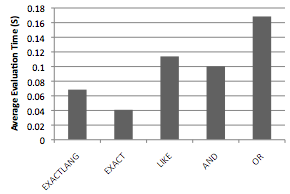
\includegraphics[width=0.7\textwidth]{p9.png}
\caption{State 2 with two transition queries Q1 and Q2. In this example, the attribute query $q_A$ is the same in both queries.} 
\end{figure} 

Notice that our transition query contains just two components. We decided to make this definition because it is coherent with our definition of ambiguity, i.e., since we assume that there are no duplicates, two instances with the same name most be distinct. Therefore, there is always an discriminative attribute/value pair that distinguish them, which can be captured by the class component. Otherwise, they cannot be distinguished by any technique. Consequently, we can always formulate a query with two components that selects uniquely an instance; however, not all queries with these two components selects only one instance. Observe that an attribute query is an approximate query that may select more than one element because of its threshold, even for a restrictive class component.  For instance, the query q = $Q_a$(label, title, "republic of chile", $\delta$) $\land$ $Q_c$(type,Country) may select all countries that contains the word "republic of", for a low value of the threshold $\delta$.

Fig. 6 depicts two instances that can be distinguished between a geographic location and a concept and Fig. 11 depicts two instances that cannot be distinguished. 

\begin{figure} 
\centering
\includegraphics[width=0.8\textwidth]{p10.png}
\caption{Two distinct instances, distinguisible.} 
\end{figure} 

\begin{figure} 
\centering
\includegraphics[width=0.8\textwidth]{p11.png}
\caption{Two distinct instances, indistinguishable.} 
\end{figure} 


\subsection{Cost Function} 
 
The heuristic search uses a distance-plus-cost heuristic function (usually denoted by f(n)) to determine the order in which the search visits states in the search space. At each iteration, it expands the state that has the minimum f(n) to the goal node. 

The f(n) is a sum of two functions, which can be denoted as f(n) = g(n) + h(n). The g(n) is the path-cost function, which is the cost from the starting node to the current node n. The heuristic h(n) is an admissible "heuristic estimate" of the distance to the goal. In other words, a heuristic h(n) is admissible if it never overestimates the cost of reaching the goal. For example, a straight line between two points is a admissible heuristic for a shortest-path problem. To guarantee the optimal path to the goal, the f(n) must be admissible and monotone (or consistent). This property is important because if it is valid, then the heuristic search (A*) will always find an optimal solution

We will now introduce our definition of h(n) and g(n) and later we will demonstrate how this model generates optimal candidate sets. 

\subsubsection{Heuristic Function} 
An admissible heuristic in our case is to assume h(n) as the minimum number of instances necessary to produces optimal candidate sets for all instances in $S_c$. In this case, we need each candidate set with exactly one instance, which in total sum up $|S_c|$ instances, i.e., one target instance per source instance.

\begin{definition}[Heuristic Function] The heuristic function is defined such as: h(n) = $|S_c| - |N|$, where N is the number of candidate set processed at the state n.
\end{definition}   

This heuristic guides the search to select always the transition that produces the smaller candidate set. 

\subsubsection{Transition Cost} Each transition has its own cost, which is the cost to evaluate the query q associated to the transition (Definition 8).

\subsubsection{Path Cost} The path-cost function g(n) is defined such as:

\[
g(n) = \sum_{i=1}^{|n|} q_i(s_i) \text{, where $q_i$ is the query selected at the state i.}
\]
 
Notice that both h(n) and g(n) have the same dimension, the cardinality of the candidate sets. In this model, the heuristic search will always select the path that produces the minimal number of elements in the candidate set, given the set of available transitions.
   
So far, we only defined the heuristic search to find the minimal candidate sets given a set of transitions; however, this model does not minimize the number of queries evaluated. In the next session, we will show we can approximate this problem to a minimal solution.



 